\documentclass[conference]{IEEEtran}
\IEEEoverridecommandlockouts
\usepackage{cite}
\usepackage{amsmath,amssymb,amsfonts}
\usepackage{graphicx}
\usepackage{textcomp}
\usepackage{xcolor}
\usepackage{booktabs}
\usepackage{array}
\def\BibTeX{{\rm B\kern-.05em{\sc i\kern-.025em b}\kern-.08em T\kern-.1667em\lower.7ex\hbox{E}\kern-.125emX}}

\begin{document}

\title{A Rule-Enhanced Personalised Training Agent for Substation Operation and Maintenance}

\author{\IEEEauthorblockN{Author One, Author Two, Author Three}
\IEEEauthorblockA{\{Affiliation, City, Postcode, China\}\\ \{corresponding author e-mail\}}}

\maketitle

\begin{abstract}
Training for substation operation and maintenance is constrained both by safety regulations and by large differences in individual competence. Fixed courseware cannot adapt to individuals, general-purpose large language models fabricate clauses and produce conclusions that cannot be traced, and retrieval-augmented generation supplies textual evidence without judging whether a recommendation itself is compliant. This paper presents a rule-enhanced personalised training agent in which safety and business-threshold decisions are delegated to a declarative rule base while the model is confined to narrative expression. The system is organised into rule configuration, rule evaluation and decision governance. Rules are stored as JSON condition trees and support group convergence, fact references and hot updates. Model output must pass four checks on structure, factual consistency, data permission and safety, and falls back to the rule path with a recorded reason otherwise, while every execution links the fired rules, the generated advice and the human decision under one run identifier. The model side fine-tunes Qwen2.5-3B-Instruct with 4-bit QLoRA on a single 8 GB GPU. On 150 structured profiles and 450 rule executions the rule set covers every profile, the number of missed failing examinations and missed competence gaps is zero, all 200 parameter-grid cases produce the correct tier, keyword supplement and severity merge, repeated executions are byte-identical, and a single evaluation takes 0.012 ms on average. On 26 held-out samples the model satisfies the output contract, factual consistency, schedule monotonicity and numeric traceability, with a median end-to-end latency of 105 s. The results show that the architecture produces individualised advice with a guaranteed safety boundary and traceable conclusions, and suits industrial training where competence is graded, thresholds are enumerable and advice requires human confirmation.
\end{abstract}

\begin{IEEEkeywords}
substation operation and maintenance, personalised training, large language model, declarative rule engine, output contract, parameter-efficient fine-tuning
\end{IEEEkeywords}
\section{Introduction}

Substation operation and maintenance (O\&M) covers equipment inspection, switching operations, condition monitoring and fault handling. Every step is bounded by safety regulations expressed as prohibitions and quantitative thresholds, such as gas concentration limits or the requirement that a switching order be checked and witnessed. Training therefore has to do more than transfer knowledge: it must make trainees form compliant judgements in a concrete working situation.


Trainees differ along four axes. Qualification levels recorded on certificates may differ from the authorisation threshold of a key task; practical performance, measured by the ratio of actual to planned duration and by whether the standard operating procedure (SOP) was followed, reflects proficiency and working habits; examination results reveal different weak knowledge points within the same post; and safety records distinguish authorised violations such as working without a permit or without a witness from ordinary deductions. This information is scattered across personnel, training, practical-task and safety ledgers, and cannot directly support an individual training decision.


Most existing training systems follow a course-examination-credit loop. They manage resources, record scores and count credits, but fail in three respects. Learning paths are arranged per post, so an individual gap in one competence item cannot be expressed. Conclusions are reported as scores and rankings without an evidence chain, so a manager cannot tell why an item of advice was produced. And advice and execution are not closed: whether advice was accepted, and what happened afterwards, is never recorded.


Large language models (LLMs) offer a new route to case generation, regulation question answering and learning advice, and have been applied to knowledge embedding and decision support in power grid dispatching [23], [24]. Used directly in a safety-critical training setting, however, they raise three risks. Clause hallucination: a model may state a non-existent clause or threshold with full confidence [9], [22]. Untraceable conclusions: numbers such as a pass mark cannot be traced to any data source. Unstable output: the same input may yield different conclusions across calls, which conflicts with assessment and audit. Retrieval-augmented generation (RAG) mitigates the first risk by supplying external knowledge [1], [11], but the retrieved text is only context for generation; it does not adjudicate the recommendation, which may still contradict the text that was retrieved.


This paper starts from a simple position: the adjudication of safety and business thresholds should not be delegated to the linguistic capability of a model, but to rules that are auditable and reproducible. The model should turn a structured conclusion into readable training advice and cover what rules cannot enumerate. We therefore build a rule-enhanced personalised training agent. The contributions are:


\begin{itemize}

\item \textbf{Architecture.} Rule configuration, rule evaluation and decision governance are separated, and the rule path and the model path are isolated by a binary `source` contract, so replacing the model touches neither the API, the data-transfer objects nor the front end.

\item \textbf{Rule modelling.} Conditions are JSON trees over a whitelisted operator set. Group convergence and per-group hit limits keep tier assignment and keyword supplementation independent, and `*\_from` references let one rule serve many objects. Thresholds are always referenced from facts rather than written as literals, so a change of business definition cannot silently invalidate a rule.

\item \textbf{Reliability.} Model output passes four checks on structure, factual consistency, data permission and safety, otherwise the system falls back to the rule path and records why. One run identifier links the fired rules, the generated advice and the human decision, so a conclusion can be explained down to a rule identifier and a data point.

\item \textbf{Evidence.} 450 rule executions and 200 grid cases on 150 structured profiles, plus 26 samples measured against the live inference service, quantifying the rule path and the model path in determinism, latency and explainability.

\end{itemize}

Section II analyses four existing routes. Section III describes the architecture and the rule engine. Section IV details the rule set, fact adaptation, output contract, corpus and fine-tuning. Section V reports experiments, Section VI discusses applicability, and Section VII concludes.


\section{Existing Routes and Their Limitations}

The decisive question for a training technology in this domain is when, and by what mechanism, a constraint is enforced. Along that axis existing work falls into four families; knowledge graphs and rule engines form two branches of the structured-knowledge family, the former supplying structure and the latter adjudication.


\subsection{A. Fixed Courseware}

Courses are authored by teaching staff, studied in sequence and assessed by examinations, with scores and credits recorded. Content is reviewed, so correctness is assured and deployment is cheap. The constraint, however, lives at authoring time and never enters run time. If an employee's real gap is moving one competence item from L2 to L3, the system can only push the same course to the whole shift. Once a regulation is revised, courses and items must be rewritten.


\subsection{B. General-Purpose LLM Agents}

An agent that decomposes tasks through tool calls adapts well to case generation and regulation questions [3], [4], and decoding strategies such as self-consistency stabilise output to some extent [20]. Three problems remain. Hallucinated clauses are stated in the same tone as correct ones [9], [22]; numbers such as pass marks, headcounts or amounts cannot be sourced; and repeated calls may disagree, which is incompatible with assessment and audit. Alignment techniques reduce but do not eliminate these failures [5], [6].


\subsection{C. Retrieval-Augmented Generation}

RAG separates retrieval from generation and attaches textual evidence, lowering hallucination markedly [1], [11]. Its constraint is still soft: the retriever finds relevant passages, but nothing prevents the generator from contradicting them. In this domain, ``the regulation was retrieved'' and ``the advice does not violate it'' are different judgements; the latter needs an explicit condition evaluation that retrieval does not provide.


\subsection{D. Knowledge Graphs and Rule Engines}

Knowledge graphs describe posts, courses and knowledge points as entities and relations, and have been used for adaptive assessment in substations [25]. Their structure is explicit and queryable. Complementary work models learners directly: deep knowledge tracing and its combination with LLMs estimate mastery per knowledge point and drive recommendations [16], [17], [19], with recent surveys mapping the area [18]. Both answer ``how well is this item mastered'' but not ``which action should a given threshold trigger'', which still requires a separate decision rule; moreover, ontology construction and instance validation depend on domain experts, so coverage is bounded by graph completeness. Rule engines built on Rete matching [14] adjudicate at run time and offer the best determinism and auditability, but their rule base degrades quietly: thresholds drift away from business definitions and rules shadow each other into unreachability, producing no error, only a falling hit rate.


\subsection{E. Positioning}

Table I compares the routes by where the constraint is enforced. Fixed courseware enforces it at authoring time, LLM agents in the prompt, RAG by demoting it to context, knowledge graphs supply structure but no adjudication, and rule engines adjudicate but offer little expression or maintenance support. This work assigns rigid safety and business decisions to the rule engine, narrative expression and unenumerable content to the fine-tuned model, and the trade-off between them to four checks that also preserve evidence. The separation is essentially one between the right to adjudicate and the right to express.


\begin{table}[t]
\caption{How each route enforces a constraint, and its main shortcoming in this domain.}
\centering
\footnotesize
\begin{tabular}{@{}p{0.190\columnwidth}p{0.267\columnwidth}p{0.340\columnwidth}p{0.158\columnwidth}@{}}
\hline
\textbf{Route} & \textbf{Constraint enforced at} & \textbf{Main shortcoming} & \textbf{Ref.} \\ \hline
Fixed courseware & Authoring time & One path per post; courses must be rewritten after each revision & --- \\
LLM agent & Prompt & Clause hallucination; untraceable numbers; unstable output & [3], [4], [20] \\
RAG & Retrieved context & Evidence without adjudication; text may contradict its source & [1], [11] \\
Knowledge graph & Ontology relations & Expert-built; coverage limited by graph completeness & [25] \\
Rule engine & Condition matching at run time & Deterministic, but drifts silently without auditing & [14] \\
This work & Declarative rules + model + four checks & Rules need maintenance; model path is slow & --- \\
\hline
\end{tabular}
\end{table}

\section{System Architecture}

\subsection{A. Design Constraints}

Four constraints shaped the design; the first three are business requirements and the fourth comes from the deployment environment:


\begin{itemize}

\item Role boundaries: employees see their own data, team leaders their team, management aggregates across the company, and administrators configure and audit the platform without taking part in decisions.

\item Sensitive data: psychological and care-related records are visible only to the employee concerned.

\item Safety first: a safety failure has veto power in any talent decision.

\item Single database: one database instance, no external rule framework and no object-relational mapper.

\end{itemize}

The fourth constraint rules out frameworks such as Drools and forces rules into JSON columns. The cost is a loss of expressiveness in the rule language; the benefit is a short deployment chain and rule changes that need neither recompilation nor release.


\subsection{B. Three Layers}

The system separates rule configuration, rule evaluation and decision governance (Fig. 1). A scene-specific adapter assembles facts from business tables; the engine loads the rules of that scene whose `enabled` flag is 1, evaluates them in descending priority and converges by group; the merged conclusion is written as a suggestion and enters the decision log after human confirmation. Two invariants are enforced in code rather than by convention: the engine writes only `rule\_result` and never modifies business data, and every outgoing suggestion carries `need\_human\_confirm = true`. Neither has a configuration switch, so the agent can only advise.


\begin{figure}[!t]
\centering
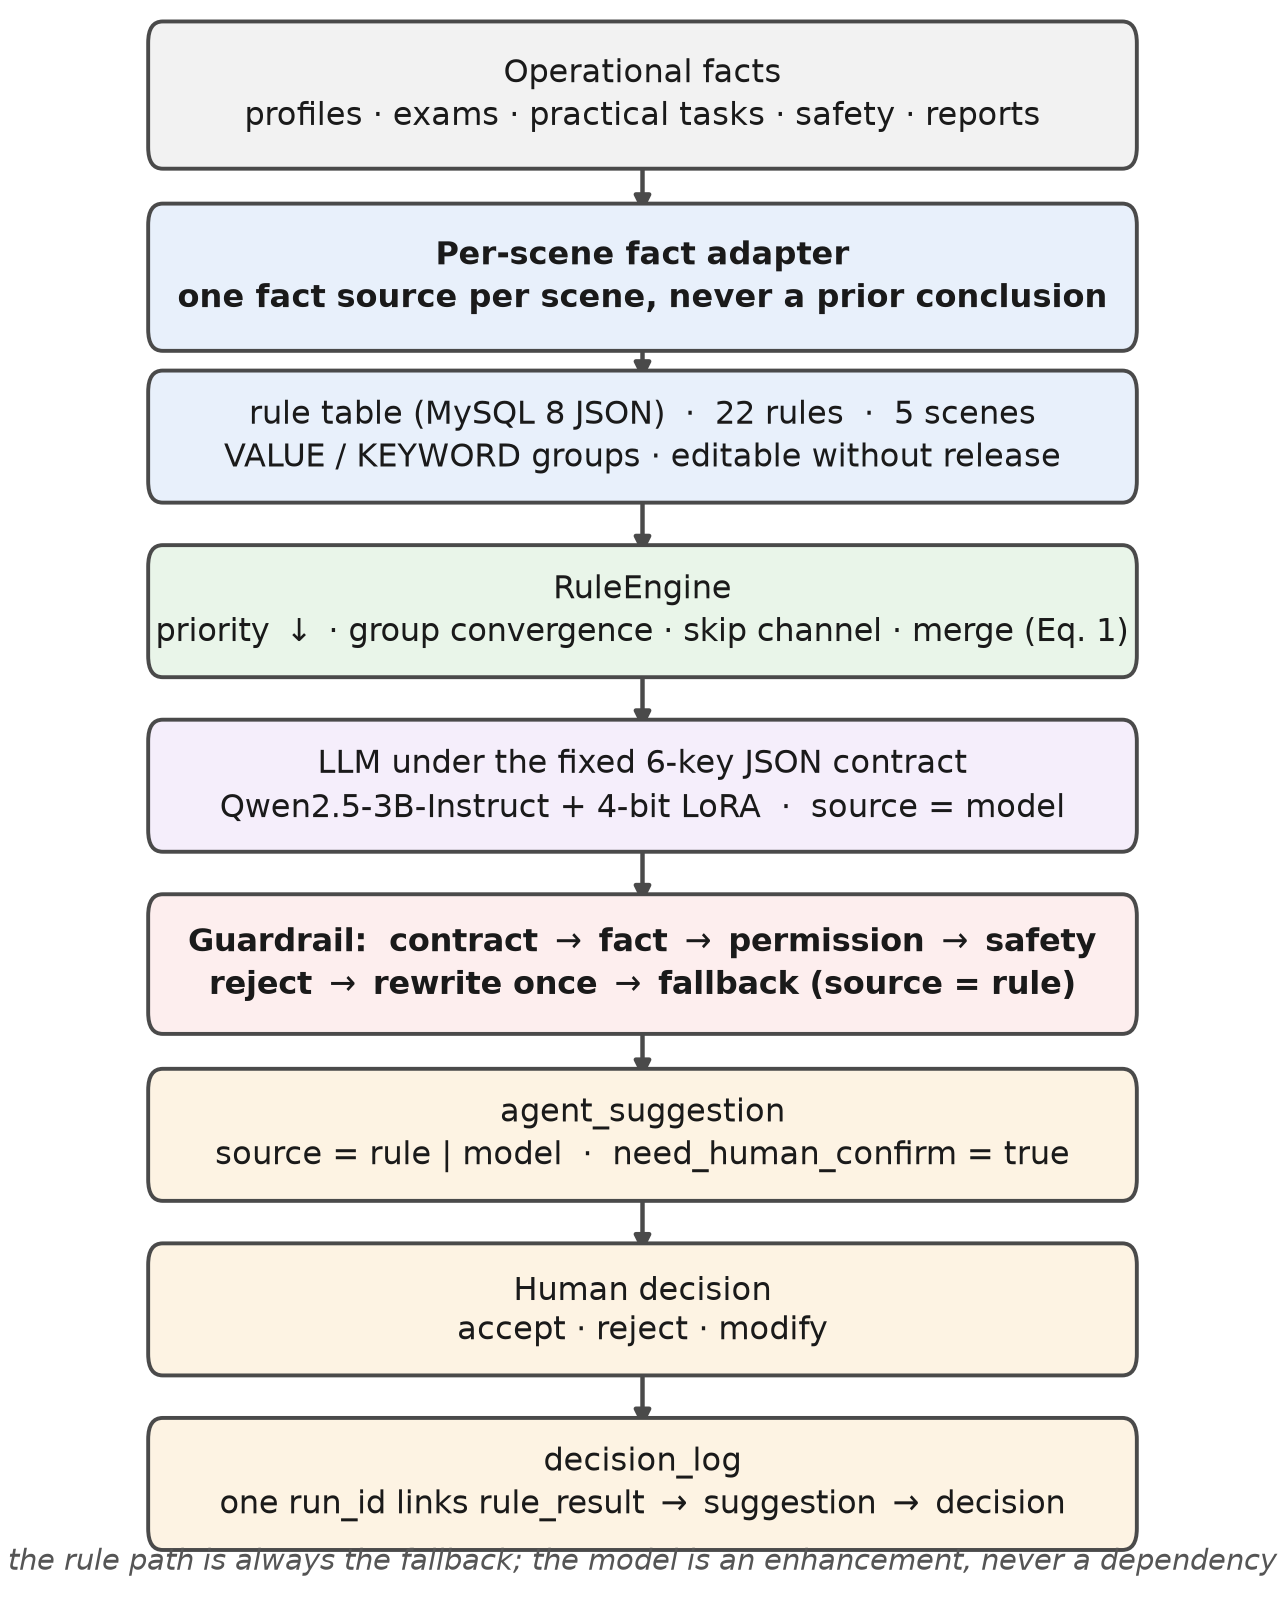
\includegraphics[width=\columnwidth]{fig1_architecture}
\caption{System architecture. The rule layer adjudicates safety and business thresholds, the evaluation layer records fired rules and skip reasons, and the decision layer records human dispositions.}
\label{fig1}
\end{figure}

\subsection{C. Declarative Rule Engine}

A rule is one row of the `rule` table. Groups let tier assignment and keyword supplementation be judged independently, and `max\_hits` caps the number of hits within a group. `condition\_json` is a pure data structure: no script, no expression evaluation, no concatenated SQL, so rule content is treated as untrusted input. Conditions that cannot be decided, whether because the operator is unknown, a fact is missing or a type does not match, enter a skip channel with a recorded reason; they are neither counted as hits nor allowed to abort the run.


Evaluation loads the rules of the scene whose `enabled` flag is 1, sorts them by priority and then by rule code, and walks the list. Each condition returns true, false or unknown; unknown conditions record a skip reason and continue. A hit whose `stop\_on\_match` flag is set closes its own group, a group that reaches `max\_hits` is closed as well, and closed groups are skipped for the remainder of the run. Convergence therefore acts on groups rather than on the scene, so the default group keeps the original semantics of stopping at the first high-priority hit, while the safety and tier groups decide independently. Because sorting is normalised, the result does not depend on physical row order, and because every non-hit leaves a reason, replay analysis can treat ``not fired'' as data. Multiple hits are merged by


\begin{equation}\mathit{s} ^{ \mathrm{*} }  =  \mathit{s} _{ \mathrm{j} } ,   j = arg max _{ \mathrm{h $\in$ H} }  rank( \mathit{s} _{ \mathrm{h} } )\label{eq1}\end{equation}

where rank(low) < rank(medium) < rank(high); actions and causes are de-duplicated in hit order and the primary cause is the first hit. If nothing matches, the engine returns `matched = false` with a reason instead of raising, so batch replays always complete.


\subsection{D. Guardrails and Fallback}

Model output must pass four checks before acceptance: structural contract, factual consistency, data permission and safety rules. The order follows increasing cost, so invalid model calls and data access are avoided. Formally,


\begin{equation}\mathit{y}  =  \mathit{f} _{ \mathrm{model} } ( \mathit{x} )  if  \mathit{Valid} ( \mathit{x} ) = true;    \mathit{f} _{ \mathrm{rule} } ( \mathit{x} )  otherwise\label{eq2}\end{equation}

A rejected output triggers at most one bounded rewrite; if it still fails, the system returns the rule-path conclusion and writes `fallback\_note`. The single rewrite is deliberate: repeated rewriting degenerates into tacit approval. Because `source` takes only `rule` or `model`, and the three agent endpoints keep a fixed request and response shape, replacing the model requires only a new service implementation (Fig. 2).


\begin{figure}[!t]
\centering
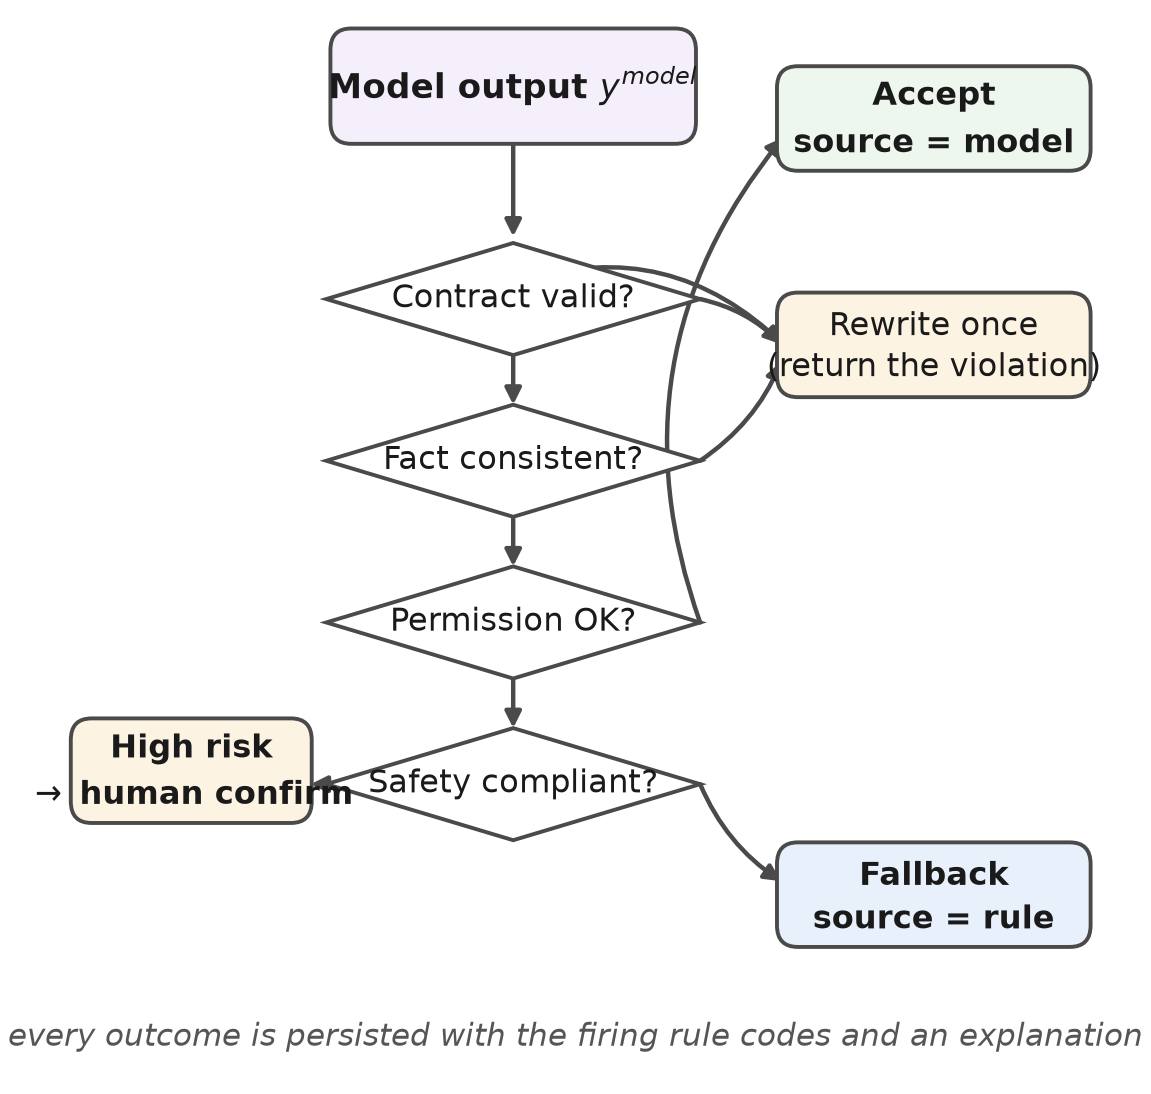
\includegraphics[width=\columnwidth]{fig2_guardrail}
\caption{Guardrail and fallback. Structure, facts and safety are checked in turn; failure triggers one bounded rewrite and then a fallback to the rule path; high-risk output always reaches human confirmation.}
\label{fig2}
\end{figure}

\section{Key Implementation}

\subsection{A. Rule Set}

The base covers five scenes with 22 rules, 20 of which are active and two retained as historical versions for tracing earlier conclusions (Table II). Two principles guide the modelling. Thresholds are referenced from facts rather than written as literals: pass marks and authorisation levels come from the fact table, so one rule serves pass marks of 80 or 85 and thresholds from L2 to L4. Composition beats enumeration: gas attribution and measures are fetched through `*\_from`, so five tier rules serve every gas type, whereas one rule group per gas would grow linearly with the gas list.


\begin{table}[t]
\caption{Rule inventory. 22 rules in five scenes, 20 of them active.}
\centering
\footnotesize
\begin{tabular}{@{}p{0.275\columnwidth}p{0.090\columnwidth}p{0.171\columnwidth}p{0.419\columnwidth}@{}}
\hline
\textbf{Scene} & \textbf{No.} & \textbf{Group} & \textbf{Rule codes and consumed facts} \\ \hline
PERSONAL\_GAP & 3 & SAFETY, default & SAFETY\_VETO\_VIOLATION, SAFETY\_DEDUCTION (safety\_risk); SKILL\_BELOW\_REQUIRED (current\_level < required\_level) \\
EXAM\_RESULT & 1 & default & EXAM\_BELOW\_PASS (score < pass\_score) \\
TALENT\_GAP & 2 & default & BACKUP\_SHORTAGE (backup\_count); FUTURE\_DEMAND\_GAP (future\_demand > current\_supply) \\
REPORT\_ANALYSIS & 2 & default & PRACTICE\_HUMAN\_CAUSE (sop\_preparation); PRACTICE\_SKILL\_CAUSE (actual\_hours\_ratio > 1.2 and skill\_missing) \\
REPORT\_GAS & 12 & VALUE (5), KEYWORD (7) & over\_threshold and $\rho$ for the five tiers; document\_text for the seven keyword rules \\
\hline
\end{tabular}
\end{table}

In the personal and practical-analysis scenes the SAFETY group ranks first: authorised violations (working beyond authority, without a permit or without a witness) are rated high and suspend independent authorisation, while ordinary deductions are rated medium and require retraining. Both rules live in the same group and do not shadow each other, because the group closes only after its first hit. The skill-gap and examination rules compare two facts and contain no literal threshold.


In the gas scene, five VALUE rules assign a tier from the margin ratio and stop at the first hit, while seven KEYWORD rules supplement causes and measures from the report text and may raise severity; the final severity is the most severe of all hits. The margin ratio is


\begin{equation}\mathit{$\rho$}  =  \frac{ \mathit{u}  −  \mathit{u} _{ \mathrm{0} } }{ \mathit{u} _{ \mathrm{max} }  −  \mathit{u} _{ \mathrm{0} } }\label{eq3}\end{equation}

with u the reading, u0 the alarm threshold and umax the instrument range. Because the sign of the ratio carries direction, the near-threshold rule must bound both sides; with an upper bound only, a negative ratio always satisfies it and the terminal rule becomes unreachable.


\subsection{B. Fact Adaptation and Personalisation}

Each scene has exactly one fact source. The adapter is deterministic and reads only business records, never earlier conclusions, so the same profile always yields the same rule references. Safety records are mapped onto three risk levels, with authorised violations at 2 and deductions at 1.


The model receives an enumerated fact list rather than raw text: ten groups numbered from F1, each tagged with its source, so that every sentence can be traced back. The tenth group is conclusive: which skills enter the gap list and which count as assets is aggregated by the backend from the skill radar, and the model only restates it. In practice the model's two typical deviations are a missing gap, contradicting its own summary, and a spurious gap, naming a skill that is not below requirement; moving the aggregation to the backend removes both. When no gap exists the source tag changes, and the prompt then imposes no coverage constraint, which would otherwise force an empty gap list.


For employee i and competence item k the post gap and the future-demand gap are


\begin{equation}\mathit{G} _{ \mathit{i} \mathrm{,} \mathit{k} }  = max(0,  \mathit{R} _{ \mathit{i} \mathrm{,} \mathit{k} }  −  \mathit{S} _{ \mathit{i} \mathrm{,} \mathit{k} } )\label{eq4}\end{equation}

\begin{equation}\mathit{F} _{ \mathit{i} \mathrm{,} \mathit{k} }  = max(0,  \mathit{D} _{ \mathit{i} \mathrm{,} \mathit{k} }  −  \mathit{S} _{ \mathit{i} \mathrm{,} \mathit{k} } )\label{eq5}\end{equation}

where R is the post requirement, D the planned future requirement and S the demonstrated level; the three are not interchangeable. The reinforcement score adds normalised deviations of examination, practice, certificate and safety to the two gaps,


\begin{equation}\mathit{Pr} _{ \mathit{i} \mathrm{,} \mathit{k} }  =  \mathit{w} _{ \mathrm{1} } \mathit{G} _{ \mathit{i} \mathrm{,} \mathit{k} }  +  \mathit{w} _{ \mathrm{2} } \mathit{F} _{ \mathit{i} \mathrm{,} \mathit{k} }  +  \mathit{w} _{ \mathrm{3} } \mathit{E} _{ \mathit{i} \mathrm{,} \mathit{k} }  +  \mathit{w} _{ \mathrm{4} } \mathit{Q} _{ \mathit{i} \mathrm{,} \mathit{k} }  +  \mathit{w} _{ \mathrm{5} } \mathit{C} _{ \mathit{i} \mathrm{,} \mathit{k} }  +  \mathit{w} _{ \mathrm{6} } \mathit{A} _{ \mathit{i} \mathrm{,} \mathit{k} }\label{eq6}\end{equation}

and is mapped onto three tiers,


\begin{equation}\mathit{p} _{ \mathit{i} \mathrm{,} \mathit{k} }  =  \mathit{P1}   if  \mathit{Pr} _{ \mathit{i} \mathrm{,} \mathit{k} }  $\ge$  \mathit{$\theta$} _{ \mathrm{1} } ;    \mathit{P2}   if  \mathit{$\theta$} _{ \mathrm{2} }  $\le$  \mathit{Pr} _{ \mathit{i} \mathrm{,} \mathit{k} }  <  \mathit{$\theta$} _{ \mathrm{1} } ;    \mathit{P3}   otherwise\label{eq7}\end{equation}

rendered as P1 to P3 in the interface. Weights and thresholds are configuration, so a site that values certificate validity or safety exposure differently can change them without code changes.


\subsection{C. Output Contract}

The model writes six keys (Table III); identifiers, timestamps, source labels, evidence counts and the confirmation flag are filled by the backend. This division is what makes the four checks tractable: structure is owned by code and narrative by the model, so the verification boundary is exact. A number not present in the fact list does not invalidate the conclusion; it is recorded in `unverified\_numbers` and the confidence is capped at 0.6, which flags it for review.


\begin{table}[t]
\caption{The six-key output contract written by the model. All other fields are filled by the backend.}
\centering
\footnotesize
\begin{tabular}{@{}p{0.241\columnwidth}p{0.122\columnwidth}p{0.592\columnwidth}@{}}
\hline
\textbf{Key} & \textbf{Type} & \textbf{Constraint} \\ \hline
summary & string & Non-empty; assets first, then the main gap and direction \\
confidence & number & [0,1]; capped at 0.6 when an unsourced number appears \\
verdict & object & headline non-empty; reasons $\ge$ 1, each citing a fact identifier \\
gaps & array & $\ge$ 1 item with skill, current, required, future, severity, priority, impact, action; severity $\in$ \{HIGH, MEDIUM, LOW\}; priority $\in$ \{P1, P2, P3\}; levels $\in$ [1,5]; skills unique \\
plan & array & $\ge$ 1 step; step ascending; kind $\in$ \{course, mentoring, mock exam\}; to\_level = L[1-5]; due\_at = YYYY-MM-DD and later than today \\
compound\_path & object & title, why, benefit non-empty; stages $\ge$ 1 with phase, focus, skills, milestone \\
\hline
\end{tabular}
\end{table}

\subsection{D. Corpus Reconstruction and Fine-Tuning}

The first corpus paired a fixed instruction with a prose profile and an eleven-key target, 150 samples in all. Connecting it to the live service exposed three mismatches. The prompt differed: the corpus concatenated basic information, examination results and mentor comments, whereas the service sends a four-part prompt with a date, an enumerated fact list, a gap list and an output template. The contract differed: the service expects six keys, and only `gaps` shared a name with the eleven-key schema, so none of the 150 targets passed validation. And the answers were incomplete: the median answer was 1795 tokens while the first run used a 1024-token window, truncating about 78\% of answer tokens.


The second corpus contains 500 samples. The generator reproduces the four-part prompt verbatim from the server source, using profiles only as a fact source; each sample samples a fresh combination of facts, with 124, 232 and 144 samples carrying one, two and three gaps, both passing and failing examinations represented, and 49 posts covered. Four self-checks on contract, numbers, style and rules gate admission. The median sample is 3432 tokens, the 95th percentile 3806 and the maximum 3924, so the window is set to 4096. The first corpus needed only 2368 tokens in total, yet was truncated at 1024, showing that answer share rather than total length is the binding constraint. The second corpus also yields shorter answers, 1069 against 1795 tokens, because the six-key structure drops three overlapping narrative sections.


Fine-tuning runs on one 8 GB GPU with 4-bit double quantisation, training only the seven projection layers at a 4096 window, an effective batch of 8, a learning rate of 1e-4 with cosine decay, and 300 steps over five epochs in 7.6 h. Trainable parameters are 29.9 M, 0.96\% of the base model. Training loss falls from 11.56 at step 5 to 0.063 at step 300, averaging 0.577; validation loss falls monotonically from 0.0198 to 0.0106 and flattens after step 200. The first logged value is close to the entropy of a uniform distribution over the vocabulary, ln 151936 = 11.93, which we read as warm-up rather than as a quality indicator. Validation loss is lower than the final training loss mainly because the two sets share a source, so it reflects template reproduction rather than generalisation; loss is also insensitive to structural properties such as whether the gap list matches or the schedule increases. Model quality is therefore measured on outputs, not on loss.


\section{Experiments}

\subsection{A. Setup}

Training, inference, serving and evaluation run on one machine: Windows 11, an Intel Core i7-14650HX with 32 GB of memory, an NVIDIA RTX 5060 Laptop GPU with 8 GB, OpenJDK 17.0.18, Spring Boot 3.5.16 and MySQL 8.4. Model serving uses the LLaMA-Factory api mode behind an OpenAI-compatible endpoint with temperature 0.2 and `response\_format = json\_object`, which is the same setting the backend uses in production. The corpus contains 150 profiles generated by a factorial design, with 25 records per safety class and 6 records per examination score, so every class is represented; it is intended for internal consistency and coverage, not as a replication of the workforce distribution of any particular utility.


\subsection{B. Protocol}

Four protocols are used and are not interchangeable. Rule replay extracts the rule definitions from the deployment scripts, converts profiles into scene facts and executes the documented DSL semantics, 450 times in total; each case is run twice and the physical rule order is reversed to test determinism. Grid verification exercises 200 gas cases for tier assignment, hit limits, severity merge and fact references. Corpus validation applies the live six-key checks to the 150 targets of the first corpus. Model measurement sends 20 held-out prompts with no textual overlap with training, plus 6 verbatim samples as a control.


\subsection{C. Rule-Set Effectiveness}

Coverage is the share of profiles hit by at least one rule,


\begin{equation}\mathit{C}  =  \frac{ |\{  \mathit{i}  : ∃  \mathit{r}  $\in$  \mathit{R} ,  \mathit{fired} ( \mathit{i} ,  \mathit{r} ) \}| }{ \mathit{N} }\label{eq8}\end{equation}

where N is the number of profiles, R the rule set and fired(i, r) indicates whether profile i triggers rule r. Of 450 executions 404 matched and all 150 profiles received at least one recommendation (Table IV, Fig. 3). Per scene, the personal diagnosis scene matched 145 times (96.7\%), the examination scene 132 (88.0\%) and the practical-analysis scene 127 (84.7\%).


\begin{table}[t]
\caption{Rule-set coverage and semantic verification. Coverage is measured on 150 profiles; semantics on 200 grid cases.}
\centering
\footnotesize
\begin{tabular}{@{}p{0.444\columnwidth}p{0.266\columnwidth}p{0.245\columnwidth}@{}}
\hline
\textbf{Item} & \textbf{Result} & \textbf{Rate} \\ \hline
Profiles hit by at least one rule & 150 / 150 & 100\% \\
Executions matched (personal / exam / report) & 145, 132, 127 of 150 & 96.7, 88.0, 84.7\% \\
Failing examinations detected & 132 / 132 & 100\% \\
Competence gaps detected & 120 / 120 & 100\% \\
Profiles with a safety record handled & 125 / 125 & 100\% \\
Tier, keyword supplement, severity merge, fact reference & 200, 200, 200, 120 & 100\% each \\
Unreachable rules & 0 & --- \\
\hline
\end{tabular}
\end{table}

Two business-level checks follow. Of the 132 profiles below the course pass mark, all were matched, with no misses and no false positives, giving 100\% recall and 100\% precision against the business pass line. Of the 120 profiles whose certificate level is below the authorisation threshold, all were matched; a further 25 profiles triggered the safety group alone, giving 145 matches in total. Of the 125 profiles carrying a safety record, all were explicitly handled by the safety group, including the 75 authorised violations, leaving no safety record unprocessed. On the 200-case grid, tier assignment is correct under both definitions of the margin ratio, the terminal rule `REPORT\_GAS\_WITHIN` fires on all 40 comfortable cases, no comfortable case is escalated to medium, and keyword supplementation, severity merge and fact references are all correct. Every active rule fires at least once, so there is no unreachable rule.


\begin{figure}[!t]
\centering
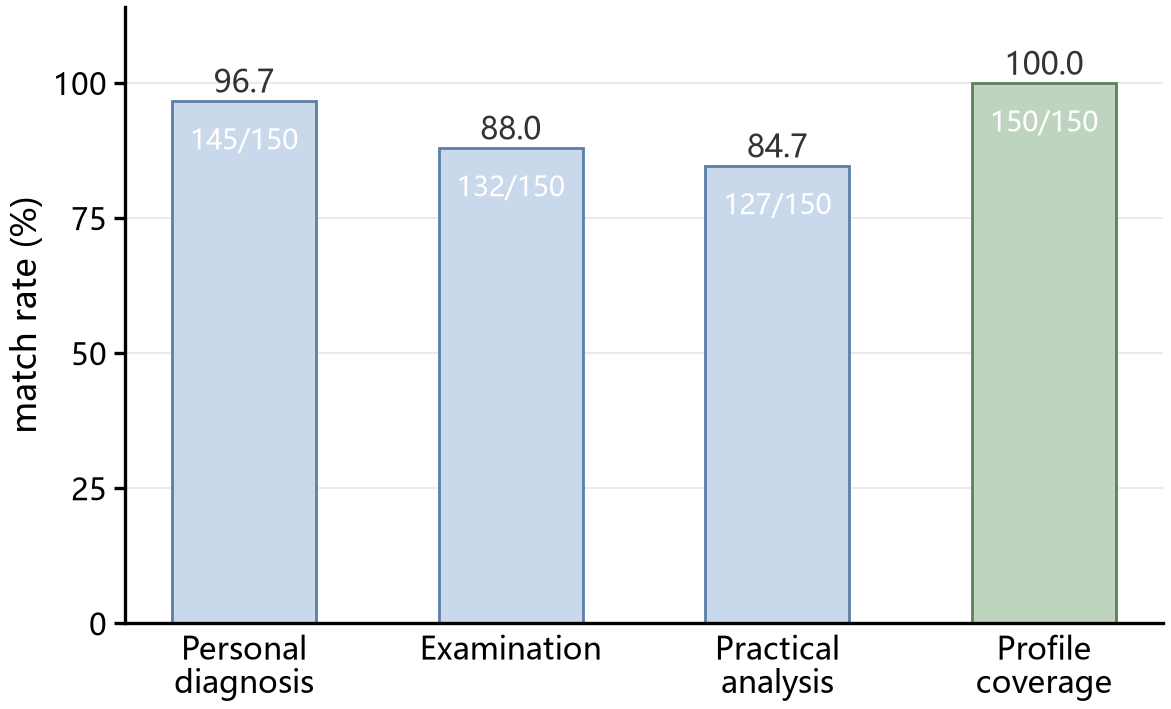
\includegraphics[width=\columnwidth]{fig3_coverage_en}
\caption{Match rate per scene and profile-level coverage. The three scenes reach 96.7\%, 88.0\% and 84.7\%; every profile is hit by at least one rule.}
\label{fig3}
\end{figure}

\subsection{D. Determinism and Latency}

Repeated executions are byte-identical in all 450 cases, and reversing the physical rule order leaves conclusions unchanged, because sorting is normalised by priority and rule code. A single in-process evaluation takes 0.0122 ms on average and 0.0194 ms at the 95th percentile; this excludes database access, fact assembly, model inference and network round trips, and is not an end-to-end figure. The model path shows a median of 105.4 s, a mean of 124.3 s and a maximum of 324.7 s for the 3B model under 4-bit quantisation at a 4096 window, while the front end called the same service concurrently. The two paths differ by about seven orders of magnitude (Fig. 4). That gap cannot be tuned away, and it fixes the deployment form: the model path must be asynchronous, fallback-capable and backed by the rule path, and cannot sit on any synchronous interaction chain.


\begin{figure}[!t]
\centering
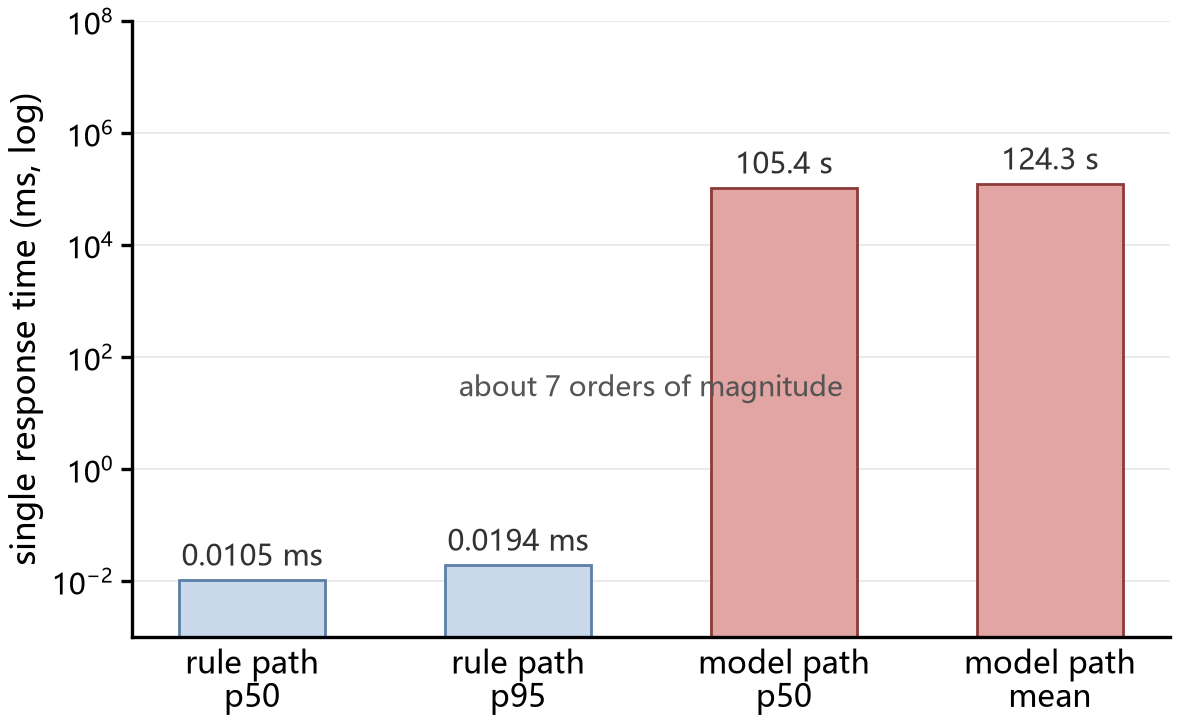
\includegraphics[width=\columnwidth]{fig4_latency_en}
\caption{Single-response time on a logarithmic scale. The rule path is shown at its 95th percentile and the model path at its median.}
\label{fig4}
\end{figure}

\subsection{E. Model Output Quality}

On 20 held-out samples every output is valid JSON and satisfies the six-key contract. The gap set equals the gap list, the three levels agree with the fact list item by item, severity agrees with the radar priority, and every schedule falls after the current date and increases strictly. Every reason cites a valid fact identifier, with 4.75 distinct facts cited on average; all numbers are traceable and the safety boundary appears in every output. Ten checks under the contract pass on all 26 samples, and the verbatim control behaves the same, so the model does not depend on remembering particular prompts (Table V).


\begin{table}[t]
\caption{Measured model compliance on 20 held-out samples with 6 verbatim samples as control.}
\centering
\footnotesize
\begin{tabular}{@{}p{0.486\columnwidth}p{0.243\columnwidth}p{0.226\columnwidth}@{}}
\hline
\textbf{Check} & \textbf{Held-out} & \textbf{Verbatim} \\ \hline
Valid JSON and six-key contract & 100\% & 100\% \\
Gap set, levels and severity agree with the facts & 100\% & 100\% \\
Schedule later than today and strictly increasing & 100\% & 100\% \\
Reasons cite fact identifiers (mean 4.75); numbers traceable & 100\% & 100\% \\
Priority rises with gap size (contract-free check) & 80\% & 67\% \\
Latency, median / mean / max (s) & 105 / 124 / 325 & 99 / 97 / 108 \\
\hline
\end{tabular}
\end{table}

Two caveats apply. The held-out prompts do not overlap the training set textually, but the profiles come from the same 150 people and the same template, so the result measures contract compliance and factual fidelity rather than generalisation to unseen employees. And under a criterion the contract does not specify, namely that priority should increase with gap size, the model reaches 80\% while the reference outputs of the first corpus reach 75\%; the model is restating the severity-to-priority convention of the corpus, not deriving priority, which is why the criterion was left out of the contract.


\subsection{F. Comparison}

Comparing three output forms on the same corpus makes the division of labour concrete. The reference outputs of the first corpus are complete in content but inconsistent with the live contract and pass none of the six-key checks, while 74.7\% of their gap levels agree with the profile and 99.8\% of their numbers are traceable. The rule path is deterministic, fully traceable and contract-consistent at 0.0122 ms, but its expression is fixed. The measured model satisfies contract, facts, schedule and traceability at 105 s without any determinism guarantee. The three are not substitutes: rules guarantee the absence of errors, the model extends expression and coverage, and the checks arbitrate between them while preserving evidence.


\section{Applicability and Discussion}

\subsection{A. Conditions}

The approach applies best when four conditions hold together:


\begin{itemize}

\item Competence is graded: items map onto ordered levels or enumerable states, so that ``below requirement'' is decidable.

\item Thresholds are enumerable: regulatory and assessment requirements can be written as conditions and maintained as facts rather than buried in code or documents.

\item Profiles are structured: personnel, examination, practical and safety records are already stored and can be aggregated per person; if data are still paper-based, the adapter becomes the dominant cost.

\item Advice requires confirmation: the process accepts that the agent advises and a human decides, so that recommendations are reviewable and attributable.

\end{itemize}

\subsection{B. Typical Scenarios}

Within substation O\&M the architecture can be reused directly for post training and assessment, where an individual path is generated from the skill radar and a failed examination triggers error review; for practical-report attribution, which separates insufficient skill, pointing to training, from non-compliance with the SOP, pointing to process revision; for safety-record disposition, where authorised violations and ordinary deductions are handled at different levels with safety taking precedence over skill; for qualification management, where a certificate level inconsistent with the authorisation threshold yields a renewal or downgrade recommendation; and for team capability review, aggregating individual facts for backup-strength assessment. The same architecture transfers to other strongly regulated industrial training, such as dispatch operation, gas-turbine maintenance and high-voltage testing, where the migration cost lies mainly in the fact adapter rather than in the engine or the model.


\subsection{C. When Not Applicable}

Four situations call for a different design: open-domain question answering, where conditions cannot be enumerated and retrieval-augmented generation is more appropriate; settings without structured records, where the rule path would fall into the skip channel and coverage would collapse; real-time closed-loop control, where the rule path is fast enough but the model path is not, so interlocking requirements cannot be met; and fully automated execution without human confirmation, which would require the safety responsibility boundary to be reassessed.


\subsection{D. Relation to Other Routes and Limitations}

The approach complements rather than replaces knowledge graphs and RAG: a graph expresses relations and can supply finer-grained competence items, retrieval supplies textual evidence and clause citations, so the division is graph for structure, retrieval for evidence, rules for adjudication and model for expression. In the present implementation rules and model already work together, while graph and retrieval remain future work.


Three limitations remain. The study is confined to one utility and 150 profiles generated by a factorial design, so the figures should be read as a case rather than as population estimates. Model measurement uses a single sample per prompt, giving a resolution of about 4 percentage points at 26 samples, which supports order-of-magnitude statements only; confidence intervals would require a larger sample and repeated sampling. Finally, no expert ratings or field adoption data have been collected, so we make no causal claim about learning outcomes and report only coverage, semantic correctness and output compliance.


\section{Conclusion}

This paper addressed the tension between safety constraints and individual differences in substation O\&M training with a rule-enhanced personalised training agent. Safety and business decisions are delegated to a declarative rule engine, narrative expression to a fine-tuned model, and the boundary between them to four checks with fallback. Rules are stored as JSON condition trees supporting group convergence, fact references and hot updates, and thresholds are referenced from facts rather than hard-coded, so one rule adapts to different pass marks and authorisation levels.


Across 450 executions on 150 structured profiles the rule set covers every profile, misses no failing examination or competence gap, and explicitly handles all 125 profiles carrying a safety record. On 200 grid cases, tier assignment, keyword supplementation, severity merge and fact references are all correct, with no unreachable rule; repeated executions are byte-identical and a single evaluation takes 0.0122 ms. On 26 samples the fine-tuned model satisfies the six-key contract, factual consistency, schedule monotonicity and numeric traceability, citing 4.75 distinct facts on average, with a median end-to-end latency of 105 s.


The results indicate that, where competence is graded, thresholds are enumerable and profiles are structured, an architecture that assigns adjudication to rules, expression to a model and arbitration to checks can generate individualised training advice with a guaranteed safety boundary and traceable conclusions. Future work includes connecting knowledge graphs and retrieval to extend the granularity of competence items, enlarging the sample with repeated sampling to attach confidence intervals to compliance rates, and conducting expert rating and field adoption studies.


\begin{table}[t]
\caption{How each route enforces a constraint, and its main shortcoming in this domain.}
\centering
\footnotesize
\begin{tabular}{@{}p{0.190\columnwidth}p{0.267\columnwidth}p{0.340\columnwidth}p{0.158\columnwidth}@{}}
\hline
\textbf{Route} & \textbf{Constraint enforced at} & \textbf{Main shortcoming} & \textbf{Ref.} \\ \hline
Fixed courseware & Authoring time & One path per post; courses must be rewritten after each revision & --- \\
LLM agent & Prompt & Clause hallucination; untraceable numbers; unstable output & [3], [4], [20] \\
RAG & Retrieved context & Evidence without adjudication; text may contradict its source & [1], [11] \\
Knowledge graph & Ontology relations & Expert-built; coverage limited by graph completeness & [25] \\
Rule engine & Condition matching at run time & Deterministic, but drifts silently without auditing & [14] \\
This work & Declarative rules + model + four checks & Rules need maintenance; model path is slow & --- \\
\hline
\end{tabular}
\end{table}

\begin{table}[t]
\caption{Rule inventory. 22 rules in five scenes, 20 of them active.}
\centering
\footnotesize
\begin{tabular}{@{}p{0.275\columnwidth}p{0.090\columnwidth}p{0.171\columnwidth}p{0.419\columnwidth}@{}}
\hline
\textbf{Scene} & \textbf{No.} & \textbf{Group} & \textbf{Rule codes and consumed facts} \\ \hline
PERSONAL\_GAP & 3 & SAFETY, default & SAFETY\_VETO\_VIOLATION, SAFETY\_DEDUCTION (safety\_risk); SKILL\_BELOW\_REQUIRED (current\_level < required\_level) \\
EXAM\_RESULT & 1 & default & EXAM\_BELOW\_PASS (score < pass\_score) \\
TALENT\_GAP & 2 & default & BACKUP\_SHORTAGE (backup\_count); FUTURE\_DEMAND\_GAP (future\_demand > current\_supply) \\
REPORT\_ANALYSIS & 2 & default & PRACTICE\_HUMAN\_CAUSE (sop\_preparation); PRACTICE\_SKILL\_CAUSE (actual\_hours\_ratio > 1.2 and skill\_missing) \\
REPORT\_GAS & 12 & VALUE (5), KEYWORD (7) & over\_threshold and $\rho$ for the five tiers; document\_text for the seven keyword rules \\
\hline
\end{tabular}
\end{table}

\begin{table}[t]
\caption{The six-key output contract written by the model. All other fields are filled by the backend.}
\centering
\footnotesize
\begin{tabular}{@{}p{0.241\columnwidth}p{0.122\columnwidth}p{0.592\columnwidth}@{}}
\hline
\textbf{Key} & \textbf{Type} & \textbf{Constraint} \\ \hline
summary & string & Non-empty; assets first, then the main gap and direction \\
confidence & number & [0,1]; capped at 0.6 when an unsourced number appears \\
verdict & object & headline non-empty; reasons $\ge$ 1, each citing a fact identifier \\
gaps & array & $\ge$ 1 item with skill, current, required, future, severity, priority, impact, action; severity $\in$ \{HIGH, MEDIUM, LOW\}; priority $\in$ \{P1, P2, P3\}; levels $\in$ [1,5]; skills unique \\
plan & array & $\ge$ 1 step; step ascending; kind $\in$ \{course, mentoring, mock exam\}; to\_level = L[1-5]; due\_at = YYYY-MM-DD and later than today \\
compound\_path & object & title, why, benefit non-empty; stages $\ge$ 1 with phase, focus, skills, milestone \\
\hline
\end{tabular}
\end{table}

\begin{table}[t]
\caption{Rule-set coverage and semantic verification. Coverage is measured on 150 profiles; semantics on 200 grid cases.}
\centering
\footnotesize
\begin{tabular}{@{}p{0.444\columnwidth}p{0.266\columnwidth}p{0.245\columnwidth}@{}}
\hline
\textbf{Item} & \textbf{Result} & \textbf{Rate} \\ \hline
Profiles hit by at least one rule & 150 / 150 & 100\% \\
Executions matched (personal / exam / report) & 145, 132, 127 of 150 & 96.7, 88.0, 84.7\% \\
Failing examinations detected & 132 / 132 & 100\% \\
Competence gaps detected & 120 / 120 & 100\% \\
Profiles with a safety record handled & 125 / 125 & 100\% \\
Tier, keyword supplement, severity merge, fact reference & 200, 200, 200, 120 & 100\% each \\
Unreachable rules & 0 & --- \\
\hline
\end{tabular}
\end{table}

\begin{table}[t]
\caption{Measured model compliance on 20 held-out samples with 6 verbatim samples as control.}
\centering
\footnotesize
\begin{tabular}{@{}p{0.486\columnwidth}p{0.243\columnwidth}p{0.226\columnwidth}@{}}
\hline
\textbf{Check} & \textbf{Held-out} & \textbf{Verbatim} \\ \hline
Valid JSON and six-key contract & 100\% & 100\% \\
Gap set, levels and severity agree with the facts & 100\% & 100\% \\
Schedule later than today and strictly increasing & 100\% & 100\% \\
Reasons cite fact identifiers (mean 4.75); numbers traceable & 100\% & 100\% \\
Priority rises with gap size (contract-free check) & 80\% & 67\% \\
Latency, median / mean / max (s) & 105 / 124 / 325 & 99 / 97 / 108 \\
\hline
\end{tabular}
\end{table}

\bibliographystyle{IEEEtran}
% 参考文献以 \begin{thebibliography} 内联给出，便于直接编译；如需 BibTeX 可自行拆分。

\begin{thebibliography}{00}
\bibitem{b1} Lewis P, Perez E, Piktus A, et al. Retrieval-augmented generation for knowledge-intensive NLP tasks. Advances in Neural Information Processing Systems (NeurIPS), 2020, 33: 9459-9474. https://doi.org/10.48550/arXiv.2005.11401
\bibitem{b2} Hu E J, Shen Y, Wallis P, et al. LoRA: low-rank adaptation of large language models. International Conference on Learning Representations (ICLR), 2022. https://doi.org/10.48550/arXiv.2106.09685
\bibitem{b3} Yao S, Zhao J, Yu D, et al. ReAct: synergizing reasoning and acting in language models. International Conference on Learning Representations (ICLR), 2023. https://doi.org/10.48550/arXiv.2210.03629
\bibitem{b4} Wei J, Wang X, Schuurmans D, et al. Chain-of-thought prompting elicits reasoning in large language models. Advances in Neural Information Processing Systems (NeurIPS), 2022, 35: 24824-24837. https://doi.org/10.48550/arXiv.2201.11903
\bibitem{b5} Ouyang L, Wu J, Jiang X, et al. Training language models to follow instructions with human feedback. Advances in Neural Information Processing Systems (NeurIPS), 2022, 35: 27730-27744. https://doi.org/10.48550/arXiv.2203.02155
\bibitem{b6} Bai Y, Kadavath S, Kundu S, et al. Constitutional AI: harmlessness from AI feedback. arXiv preprint, 2022. https://doi.org/10.48550/arXiv.2212.08073
\bibitem{b7} Shinn N, Cassano F, Gopinath A, et al. Reflexion: language agents with verbal reinforcement learning. Advances in Neural Information Processing Systems (NeurIPS), 2023, 36. https://doi.org/10.48550/arXiv.2303.11366
\bibitem{b8} Rebedea T, Dinu R, Sreedhar M, et al. NeMo Guardrails: a toolkit for controllable and safe LLM applications with programmable rails. Proc. EMNLP 2023 (Demo), 2023. https://doi.org/10.48550/arXiv.2310.10501
\bibitem{b9} Ji Z, Lee N, Frieske R, et al. Survey of hallucination in natural language generation. ACM Computing Surveys, 2023, 55(12): 1-38. https://doi.org/10.1145/3571730
\bibitem{b10} Zhao W X, Zhou K, Li J, et al. A survey of large language models. arXiv preprint, 2023. https://doi.org/10.48550/arXiv.2303.18223
\bibitem{b11} Gao Y, Xiong Y, Gao X, et al. Retrieval-augmented generation for large language models: a survey. arXiv preprint, 2023. https://doi.org/10.48550/arXiv.2312.10997
\bibitem{b12} Qwen Team. Qwen2.5 technical report. arXiv preprint, 2024. https://doi.org/10.48550/arXiv.2412.15115
\bibitem{b13} Zheng L, Chiang W, Sheng Y, et al. LLaMA-Factory: unified efficient fine-tuning of 100+ language models. Proc. ACL 2024 (System Demonstrations), 2024. https://doi.org/10.48550/arXiv.2403.13372
\bibitem{b14} Forgy C L. Rete: a fast algorithm for the many pattern / many object pattern match problem. Artificial Intelligence, 1982, 19(1): 17-37. https://doi.org/10.1016/0004-3702(82)90020-0
\bibitem{b15} Majumder S, Dong L, Doudi F, et al. Exploring the capabilities and limitations of large language models in the electric energy sector. Joule, 2024, 8(6): 1599-1608. https://doi.org/10.1016/j.joule.2024.05.009
\bibitem{b16} Piech C, Bassen J, Huang J, et al. Deep knowledge tracing. Advances in Neural Information Processing Systems (NeurIPS), 2015, 28: 505-513. https://doi.org/10.48550/arXiv.1506.05908
\bibitem{b17} Neshaei S P, Davis R L, Hazimeh A, et al. Towards modeling learner performance with large language models. arXiv preprint, 2024. https://doi.org/10.48550/arXiv.2403.14661
\bibitem{b18} Cho Y, AlMamlook R E, Gharaibeh T. A systematic review of knowledge tracing and large language models in education: opportunities, issues, and future research. arXiv preprint, 2024. https://doi.org/10.48550/arXiv.2412.09248
\bibitem{b19} Li Z, Yazdanpanah V, Wang J, et al. TutorLLM: customizing learning recommendations with knowledge tracing and retrieval-augmented generation. Proc. 18th ACM Conf. on Recommender Systems (RecSys), 2024. https://doi.org/10.48550/arXiv.2502.15709
\bibitem{b20} Wang X, Wei J, Schuurmans D, et al. Self-consistency improves chain of thought reasoning in language models. International Conference on Learning Representations (ICLR), 2023. https://doi.org/10.48550/arXiv.2203.11171
\bibitem{b21} Xi Z, Chen W, Guo X, et al. The rise and potential of large language model based agents: a survey. arXiv preprint, 2023. https://doi.org/10.48550/arXiv.2309.07864
\bibitem{b22} Huang L, Yu W, Ma J, et al. A survey on hallucination in large language models: principles, taxonomy, challenges, and open questions. ACM Transactions on Information Systems, 2025. https://doi.org/10.48550/arXiv.2311.05232
\bibitem{b23} Yang Q B, Zhu S G, Liu D, et al. Research on key technologies for enhancing large language model capabilities in power grid dispatch and control[J]. Power Generation Technology, 2026, 47(4): 697-708. DOI:10.12096/j.2096-4528.pgt.260402.
\bibitem{b24} Liu J B, Guo Q L, Fu C, et al. Knowledge embedding of dispatch mechanism in large language models driven by regulation chain-of-thought[J/OL]. Automation of Electric Power Systems, 2025[2026-10-18]. http://aeps-info.com/aepsen/article/pdf/20250902005.
\bibitem{b25} Study on the adaptive test modelling based on knowledge graph in the domain of substation[J]. Journal of Physics: Conference Series, 2022, 2213: 012017. DOI:10.1088/1742-6596/2213/1/012017.
\end{thebibliography}
\end{document}